%%%%%%%%%%%%%%%%%%%%%%%%%%%%%%%%%%%%%%%%%%%%%%%%%%%%%%%%%%%%%%%%%%%%%%%%%%%%%
%%%%%%%%%%%%%%%%%%%%%%%%%  Ecommerce Percent Sales  %%%%%%%%%%%%%%%%%%%%%%%%%
%%%%%%%%%%%%%%%%%%%%%%%%%%%%%%%%%%%%%%%%%%%%%%%%%%%%%%%%%%%%%%%%%%%%%%%%%%%%%

\begin{figure}[h!]
	\centering
	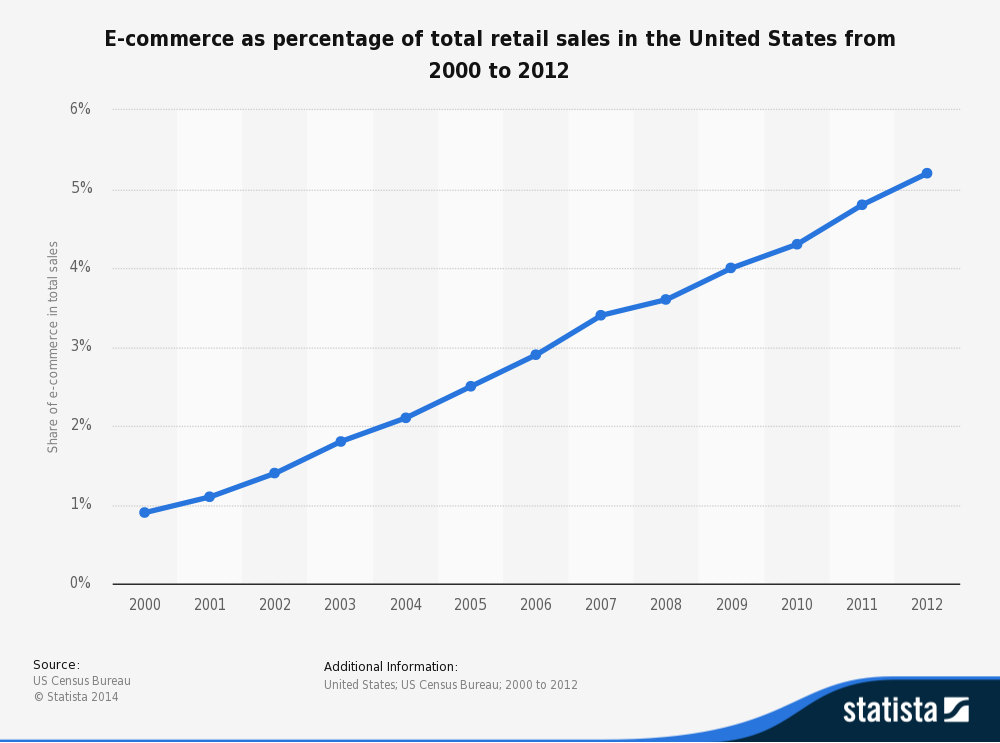
\includegraphics[width=0.7\textwidth]{figuras/ecommerce_percent.jpg}
%    \begin{tikzpicture}[y=.7cm, x=.7cm,font=\sffamily]
%        % Draw axes
%        \draw [<->,thick] (0,7) node (yaxis) [above] {$y$}
%            |- (11,0) node (xaxis) [right] {$x$};
%        %ticks
%       \foreach \x in {0,...,10}
%            \draw (\x,1pt) -- (\x,-3pt)
%            node[anchor=north] {\x};
%        \foreach \y in {0,...,6}
%            \draw (1pt,\y) -- (-3pt,\y) 
%                node[anchor=east] {\y\%}; 
%    \end{tikzpicture}
	\caption{\ecommerce como porcentaje de las ventas totales en Estados Unidos \cite{online_total_sales_2000_2012}}
	\label{figure:ecommerce_percent_sales}
\end{figure}